A sensible first case study for the \gls{qmla} framework is to prescribe a set of models, 
    where we know that the true model is among them, or at least that we would be satisfied with 
    approximating $\ho$ as the best model in the set. 
This application can be useful, for example, for expedited device calibration; 
    suppose we wish to characterise a new, \epmh{untrustued} quantum simulator/device, $S_u$, 
    and we have access to a \emph{trusted}\footnotemark \  simulator, $S_t$. 
In order to perform this calibration, 
    we treat $S_u$ as the system, $Q$, i.e. we call upon it to retrieve the datum $d$ in \cref{eqn:likelihood}, 
    where the calculation of the likelihoods for each particle are computed through $S_t$. 
If $S_u$ is reliable, the data from its calculations will be consistent with some $\ho$ of our choosing, 
    while miscalibrations will mainfest as imperfectly implemented gates/steps in the calculation of the system's likelihood, 
    and so would result in data inconsistent with $\ho$. 
Therefore, if we can prescribe the most likely miscalibrations, it may be feasible to compose a set 
    of models, $\mathbb{H}$, which represent those cases, and search for $\hp$ only within $\mathbb{H}$,
    to find identify the miscalibrations. 
For example, by encoding connections between every pair of device qubits in $\ho$, 
    we can compose models with restricted connectivity, for instance where some pairs of qubits are disconnected, 
    and hence discover whether the device allows arbitrary two-qubit gates, 
    and which pairs are disallowed. 

\footnotetext{Note: here a classical computer can fulfil the role of the trusted simulator.}


\section{Lattices}\label{sec:lattices}
We first consider $Q$ as some lattice, where \gls{qmla} attempts to identify the structure of the lattice. 
The set of viable models then comprises alternative lattices.
Due to simluation constraints, because we train models through exact unitary evolution, 
    we are restricted to $\sim~8$-qubit Hamiltonians, so we only consider lattices which can 
    be simulated in this limit. 
The \gls{es} in this chapter is then simply to propose a set of models with no further model generation, 
    with comparisons between all pairs of models through \glspl{bf}.
\par

Connectivity between lattice sites is achieved within the specific Hamiltonian formalisms
    introduced in the following sections, 
    although in general we write $\mathcal{C} = \{\bkl \}$ as the set of connected pairs $\bkl$, 
    such that the Hamiltonian for a given lattice can be thought of as 
    some function of its configuration, $\hat{H}\bk{\al, \mathcal{C}}$.
Then, we can specify candidate models only by their $\mathcal{C}$, 
    e.g. a 3-site chain can be summarised by $\mathcal{C}= \{ \langle 1,2 \rangle, \langle 2,3 \rangle\}$, 
    whereas a fully connected 3-site lattice (i.e. a triangle) is given by 
    $\mathcal{C}= \{ \langle 1, 2 \rangle, \langle 1, 3 \rangle, \langle 2, 3 \rangle\}$. 
We can then summarise the set of candidate models through the descriptions of lattice configurations, 
    corresponding to those depicted in \cref{fig:lattices}:
\begin{easylist}
    \ListProperties(Numbers=l)
    & 2-site chain
    & 3-site chain
    & 3-site fully connected (triangle)
    & 4-site fully conneted (square)
    & 4-site linearly connected (loop)

    & 4-site chain
    & 5-site chain
    & 6-site chain
    & 5-site fully connected (pentagon)
    & 6-site partially connected (grid)
\end{easylist}


\begin{figure}
    \begin{center}
        \begin{subfigure}{2.25cm}
            \begin{center}
                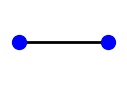
\includegraphics{theoretical_study/lattices/_2_site_chain.jpg}                        
            \end{center}
            \caption{}
        \end{subfigure}
        \qquad
        \begin{subfigure}{2.25cm} 
            \begin{center}
                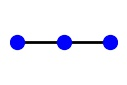
\includegraphics{theoretical_study/lattices/_3_site_chain.jpg}
            \end{center}
            \caption{}
        \end{subfigure}
        \qquad
        \begin{subfigure}{2.25cm} 
            \begin{center}
                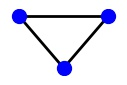
\includegraphics{theoretical_study/lattices/_3_site_lattice_fully_connected.jpg}        
            \end{center}
            \caption{}
        \end{subfigure}
        \qquad
        \begin{subfigure}{2.25cm} 
            \begin{center}
                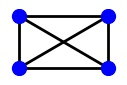
\includegraphics{theoretical_study/lattices/_4_site_lattice_fully_connected.jpg}        
            \end{center}
            \caption{}
        \end{subfigure}
        \qquad
        \begin{subfigure}{2.25cm} 
            \begin{center}
                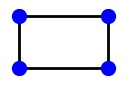
\includegraphics{theoretical_study/lattices/_4_site_square.jpg}        
            \end{center}
            \caption{}
        \end{subfigure}
        \\
        \begin{subfigure}{2.25cm} 
            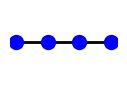
\includegraphics{theoretical_study/lattices/_4_site_chain.jpg}        
            \caption{}
        \end{subfigure}
        \qquad
        \begin{subfigure}{2.25cm} 
            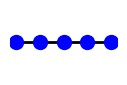
\includegraphics{theoretical_study/lattices/_5_site_chain.jpg}        
            \caption{}
        \end{subfigure}
        \qquad
        \begin{subfigure}{2.25cm} 
            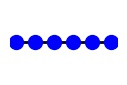
\includegraphics{theoretical_study/lattices/_6_site_chain.jpg}        
            \caption{}
        \end{subfigure}
        \qquad
        \begin{subfigure}{2.25cm} 
            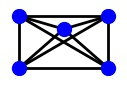
\includegraphics{theoretical_study/lattices/_5_site_lattice_fully_connected.jpg}        
            \caption{}
        \end{subfigure}
        \qquad
        \begin{subfigure}{2cm} 
            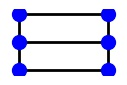
\includegraphics{theoretical_study/lattices/_6_site_grid.jpg}        
            \caption{}
        \end{subfigure}
    \end{center}
    \caption[Lattices for prescribed QMLA]{
        Lattices used for prescribed models test for \gls{qmla}.
        Lattices are characterised by the connectivity of their sites; 
            dotted lines show connection between pairs of sites.                 
    }
    \label{fig:lattices}
\end{figure}

We will use this set of lattice configurations throughout the remainder of this chapter. 

\section{Ising model}\label{sec:ising}
The Ising model is one of the most studied concepts in all of physics, 
    representing electrons on a lattice of $N$ sites, 
    where each electron can have \emph{spin} up or down 
    \cite{ising1925beitrag, onsager1944crystal, brush1967history}.
Interactions between spins $\bkl$ have strength $J_{kl}$, 
    and the transverse magnetic field acts on spin $k$ with strength $h_k$. 
It is usually stated as 
\begin{equation}
    \label{eqn:ising_standard_form}
    \hat{H}_I(\cc) = \sum_{\bkl \in \mathcal{C}} J_{kl}  \ \hat{\sigma}_k^z \ \hat{\sigma}_{l}^z + \sum_{k=1}^{N} h_k \hat{\sigma}_{k}^x.
\end{equation}

The interaction term indicates the class of magnetism of the pair's interaction, i.e. 
\begin{equation}
    \label{eqn:ising_magnetism_cases}
    \begin{cases}
        J_{kl} < 0, \ \ \textrm{ferromagnetic}; \\
        J_{kl} > 0, \ \ \textrm{antiferromagnetic}; \\
        J_{kl} = 0, \ \ \textrm{noninteracting}.
    \end{cases}
\end{equation}
If all interaction pairs are described by the same case in \cref{eqn:ising_magnetism_cases}, 
    the entire system can be said belong to that class of magnetism. 

\par 
\subsection{Note on optimising the Ising model}\label{sec:ising_optimisation}
Many treatments of the Ising model seek to find the ground state
    of the system by optimising the configuration of spins in the system. 
This involves neglecting the transverse magnetic field, and treating Ising model classically, 
    such that the ground state is found by minimising the energy function
\begin{equation}
    \label{eqn:ising_energy_function}
    E_I = \braket{\psi | H_I | \psi} = 
    \sum_{\bkl \in \mathcal{C}} J_{kl}  \ \braket{ \psi |  \hat{\sigma}_k^z \ \hat{\sigma}_{l}^z | \psi }, 
\end{equation}
    where $\ket{\psi} = \ket{\psi_1} \otimes \ket{\psi_2} \dots \otimes \ket{\psi_N}$. 

This optimisation relies on the relationship between the Ising model with its eigenvalues and eigenstates:
    \cref{eqn:ising_energy_function} consists only of $\sz$ terms, and we have that 
\begin{equation}
    \sz \ket{+} = +1 \ket{+} \ \ \ ; \ \ \ 
    \sz \ket{-} = -1 \ket{-}. 
\end{equation}

Then, for a single pair of spins $\bkl$, we have
\begin{equation}
    \label{eqn:ising_spin_cases}
    \begin{split}
        \bra{+_k \ +_l } \sz_k \ \sz_l  \ket{+_k \ +_l } =  \bra{+_k \ +_l } (+1)(+1) \ket{+_k \ +_l } = +1, \\
        \bra{+_k \ -_l } \sz_k \ \sz_l \ket{+_k \ -_l } = \bra{+_k \ -_l } (+1)(-1) \ket{+_k \ -_l } = -1 , \\
        \bra{-_k \ +_l } \sz_k \ \sz_l \ket{-_k \ +_l } = \bra{-_k \ +_l } (-1)(+1) \ket{-_k \ +_l } = -1, \\
        \bra{-_k \ -_l } \sz_k \ \sz_l \ket{-_k \ -_l } = \bra{-_k \ +_l } (-1)(1) \ket{-_k \ -_l } = +1. \\
    \end{split}
\end{equation}
So, by restricting the individual spins to $\ket{\psi_k} \in \{\ket{+}, \ket{-}\}$, 
    we can equivalently consider every spin $s_k$ in the system
    as a binary variable $s_k \in \{\pm 1\}$,
    i.e. $s_k s_l = \pm 1$ in \cref{eqn:ising_spin_cases},
    such that the energy function
\begin{equation}
    \label{eqn:ising_energy}
    E_I(\mathcal{S}) = \braket{ \psi | \hat{H}_I | \psi } = \sum\limits_{\bkl \in \cc} J_{kl} \ \ s_k s_l
\end{equation}
    can be minimised by optimising the configuration $\mathcal{S}$, when the interaction terms $\{J_{\bkl}\}$ are known.
The optimal configuration $\mathcal{S}_0$ can then be mapped to a 
    state vector $\ket{\psi_0}$, i.e. the ground state of the system. 
\par 

While this task can be greatly simplified by the reduction in \cref{eqn:ising_spin_cases}, 
    meaning we do not have to compute any unitary evolution to evaluate \cref{eqn:ising_energy},
    it is still an expensive optimisation, because effectively it is a search over $\{ \ket{\psi }\}$, 
    so the search space has $2^N$ candidates \cite{onsager1944crystal, barahona1982computational}. 
This allows for a straightforward mapping between ground state search 
    and solving combinatorial optimsiation algorithms, namely \ttt{MAX-CUT}, 
    known to be NP-complete \cite{garey1979computers}, 
    allowing for proposed advantage in mapping computationally challenging problems to quantum hardware \cite{lucas2014ising}. 
This mapping underlies ongoing research into quantum annealing as a computational platform capable of providing 
    advantage for a specific family of problems \cite{santoro2006optimization, bapst2013quantum, johnson2011quantum}. 
\par

Crucially, our goal is \emph{not} to find the ground state of $Q$, 
    but instead to find the generator of its dynamics.
Therefore, we treat the Ising \emph{quantum mechanically}:
    instead of treating \cref{eqn:ising_standard_form} as the underlying mechanism for a cost function 
    to be optimised, i.e. \cref{eqn:ising_energy}, 
    we use quantum operators and do not necessarily restrict the \gls{probe} state $\ket{\psi}$, 
    allowing us to use \cref{eqn:ising_standard_form} within the likelihood function \cref{eqn:likelihood}.

\subsection{Ising model cases}

We consider two cases: 
    firstly, where it is assumed that the strength of interactions $J_{k,l}$ are uniform (given by $J$);
    and secondly, where each interaction is assigned a unique parameter ($J_{kl}$).
In the first case, we can represent the Ising model for a given lattice configuration $\cc$ as 
\begin{equation}
    \label{eqn:ising_model_full}
    \hat{H}(\mathcal{C}) = 
        J \sum\limits_{\bkl \in \mathcal{C}} \s^{z}_{k} \s_{l}^{z} 
        + h \sum\limits_{k=1}^{N} \s^{x}_{k}, 
\end{equation}    
    allowing for the compact representation, following \cref{sec:models},
\begin{subequations}
    \label{eqn:ising_terms}
    \begin{equation}
        \vec{\alpha}_I = \irow{ J & h }
    \end{equation}
    \begin{equation}
        \terms_I = \icol{ 
            \sum\limits_{\bkl \in \mathcal{C}} \s^{z}_{k} \s_{l}^{z} \\
            \sum\limits_{k=1}^{N} \s^{x}_{k}
        }. 
    \end{equation}
\end{subequations}

In the more general second case, termed the \emph{fully parameterised} Ising model, we instead have the term set
\begin{equation}
    \label{eqn:ising_fully_parameterised}
    \termset_I = \left\{ 
        \s^{z}_{k} \s_{l}^{z}, \ \
        \sum\limits_{k=1}^{N} \s^{x}_{k}
    \right\}\limits_{\bkl \in \cc}. 
\end{equation}
    with unique parameters $J_{kl}$ associated with each interaction term $\s_k^z \s_l^z$. 
We summarise these cases in \cref{table:ising_models}.

\begin{table}[H]
    \begin{center}
        \begin{tabular}{crr}
             & $J_{\bkl}$  & $h_{k}$ \\
            \hline
            Standard & $J$ & $h$ \\
            Fully parameterised & $J_{\bkl}$ & $h_{k}$
        \end{tabular}
    \end{center}
    \caption[Types of Ising model]{Types of Ising model. Varying whether parameters $J^{z}_{\bkl}, h_k$ are shared 
        across sites gives distinct models. 
    }
    \label{table:ising_models}
\end{table}

\par 

\begin{figure}
    \begin{center}
        \QMLAfig{Nov_18/13_56/standard_ising_qhl.pdf}
    \end{center}

    \caption[\gls{qhl} for Ising model]{
        \gls{qhl} for Ising model where terms are grouped by their functionality, 
        as in \cref{eqn:ising_standard_form}. 
        (a,b) show the parameter estimates progression against 
        epochs (experiments), with the corresponding term written on top of the plot; 
        (c) shows the \gls{volume} of the parameter distribution at each epoch, as well as the 
        evolution time chosen by the \gls{edh}. 
        \figtableref
    }
    \label{fig:ising_two_param_learning}
\end{figure}

\begin{figure}
    \begin{center}
        \QMLAfig{Nov_18/13_56/fully_param_ising_qhl.pdf}        
    \end{center}
    \caption[\gls{qhl} for Ising model]{
        \gls{qhl} for fully parameterised Ising model, 
            where every interaction between pairs of sites are assigned unique parameters, 
            here neglecting the transverse field, 
            as in \cref{eqn:ising_fully_parameterised}. 
        (a)-(f) show the parameter estimates progression against 
        epochs (experiments), with the corresponding term written on top of the plot; 
        (g) shows the \gls{volume} of the parameter distribution at each epoch, as well as the 
        evolution time chosen by the \gls{edh}. 
        \figtableref
    }
    \label{fig:ising_fully_parameterised}
\end{figure}

\begin{figure}
    \begin{center}
        \QMLAfig{Nov_18/13_56/dynamics.pdf}
    \end{center}
    \caption[Ising model types' dynamics.]{
        Dynamics reproduced by Ising models under standard and fully parameterised formalisms, 
        compared with dynamics for the true system.
        \figtableref
    }
    \label{fig:ising_model_types_dynamics}
\end{figure}


We first construct models under each of these forms to verify \gls{qhl} is capable of learning in this regime. 
The former case is the standard form of the Ising model; its training is shown in \cref{fig:ising_two_param_learning}, 
    while the fully paramterised model is shown in \cref{fig:ising_fully_parameterised}. 
Ultimately, these two cases give the same Hamiltonian when $J_{\bkl} = J; \ h_k = h \ \forall k,l$.
So, the fully parameterised model will learn the same parameters as the standard Ising model,
    and we can take the \gls{bf} between them to determine which parameterisation is favourable.
Encouragingly, both models learaned the parameters to high precision, and neither model converged; 
    the \gls{volume} continues to reduce exponentially in both cases, 
    suggesting it may be impractical to seek saturation in the model training phase for every model, 
    since this may require a very large number of experiments and particles. 
\par 

The dynamics produced by both models are shown in \cref{fig:ising_model_types_dynamics}:
    the dynamics are almost indistinguishable by eye, but the standard Ising model, 
    which in this case is $\ho$, outperforms the fully parameterised model, 
    by a \gls{bf} of $10^{19}$.
This serves as a good \emph{sanity check}, confirming our expectation that 
    the \gls{bf} will favour the simpler model (i.e. fewer parameters) even when both models 
    are trained to a high precision to very similar parmaeters, and are difficult to distinguish through human intuition. 


\section{Heisenberg model}\label{sec:heisenberg}
Generalising the Ising model, the Heisenberg Hamiltonian is another model for magnetic systems consisting of a set of 
    spins on a lattice \cite{greiner2012thermodynamics}. 
It builds on the Ising model by additionally considering the spins' rotations about the $x-$ and $y-$ axes, generally stated as 
\begin{equation}
    \label{eqn:heisenberg_model_general}
    \hat{H}_H(\cc) = 
    \sum\limits_{\bkl \in \cc} J^x_{kl} \  \s^x_k \s^x_l
    + \sum\limits_{\bkl \in \cc} J^y_{kl} \ \s^y_k \s^y_l
    + \sum\limits_{\bkl \in \cc} J^z_{kl} \ \s^z_k \s^z_l
    + \sum\limits_{k=1}^{N} h_k \s^z_k.
\end{equation}

We can consider a number of formulations of the Heisenberg model, by considering whether the interaction
    parameters are completely unique for each pair of spins in each axis, 
    or  are shared by pairs of spins;
    we list the instances within the family of Heisenberg models in \cref{table:heisenberg_models}. 
\begin{table}[H]
    \begin{center}
        \begin{tabular}{crrrr}
             & $J^x_{kl}$ & $J^y_{kl}$ & $J^z_{kl}$ & $h_k$ \\
            \hline
            XXX & $J^x$ & $J^x$ & $J^x$ & $h$ \\
            XXZ & $J^x$ & $J^x$ & $J^z$ & $h$ \\
            XYZ (standard) & $J^x$ & $J^y$ & $J^z$ & $h$ \\
            Fully parameterised & $J^x_{kl}$ & $J^y_{kl}$ & $J^z_{kl}$ & $h_k$ \\
            
        \end{tabular}
    \end{center}
    \caption[Types of Heisenberg model]{
        Heisenberg model types: varying whether the interaction parameters $J^{w}_{kl}$ are shared among pairs of spins
        give distinct descriptions which are all in the family of Heisenberg models. 
    }
    \label{table:heisenberg_models}
\end{table}

Again, there are a number of possibile models to test, 
    although we can reasonably expect these to follow the same arguments as for the Ising model cases: 
    increasing generality at the expense of larger parameter dimension requires more resources to learn to a reasonable level. 
In this chapter we will refer to the Heisenberg-XYZ model,
    and will consider the fully parameterised Heisenberg model in \cref{chapter:ga};
    the parameters and terms of interest are then captured by \cref{eqn:heisenberg_terms}.


\begin{subequations}
    \begin{equation}
        \al_H = \irow{ J^x & J^y & J^z & h}    
    \end{equation}

    \begin{equation}
        \terms_H = \icol{
            \sum\limits_{\bkl \in \cc} \ \s^x_k \s^x_l \\
            \sum\limits_{\bkl \in \cc} \ \s^y_k \s^y_l \\
            \sum\limits_{\bkl \in \cc} \ \s^z_k \s^z_l \\
            \sum\limits_{k=1}^{N} \ \s^z_k  \\
        }
    \end{equation}
    \label{eqn:heisenberg_terms}
\end{subequations}


\section{Hubbard model}\label{sec:hubbard}
Another representation of solid state matter systems is given by the Hubbard model 
    \cite{hubbard1963electron, scalettar2016introduction, hubbard2013}.
The Hubbard model deals with systems of correlated fermions, 
    allowing spins to \emph{hop} between sites. 
Note the Hubbard model is synonymous with the \gls{fh} model, 
    which can be used to distinguish this model of fermions from a similar model of bosons, named the Bose-Hubbard model, 
    which is not studied in this thesis. 
We use the subscript FH to distinguish the (Fermi-)Hubbard model from the Heisenberg model $\hat{H}_{H}$, \cref{eqn:heisenberg_model_general}.
The Hubbard model is generally stated in second quantisation as

\begin{equation}
    \label{eqn:hubbard}
    \hat{H}_{FH}(\cc) = 
    \sum_{s \in \{\uparrow, \downarrow\}} \sum_{ \bkl \in \mathcal{C}} t^{s}_{\bkl} \left( \hat{c}^{\dagger}_{ks} c_{ls} + \hat{c}^{\dagger}_{ls} c_{ks} \right) 
    + \sum_{k}^{N} U_k \hat{n}\limits_{k\uparrow}\hat{n}_{k\downarrow} 
    + \sum_{k}^{N} \mu_k \left( \hat{n}\limits_{k\uparrow} + \hat{n}_{k\downarrow} \right)     
\end{equation}
    where 
\begin{easylist}[itemize]
    & $\hat{c}_{ks}$ and $\hat{c}^{\dagger}_{ks}$ are respecitvely the fermionic annihilation and creation operators for spin $s \in \{ \uparrow, \downarrow \}$ on site $k$;
    & $\hat{n}_{ks} = \hat{c}^{\dagger}_{ks} \hat{c}_{ks}$ is a counting operator to count the number of spins $s$ on site $k$;
    & $t^s_{\bkl}$ is the kinetic (hopping) term for spin $s$ between sites $k$ and $l$; 
    & $U_k$ is the onsite (repulsion) energy for site $k$;
    & $\mu_k$ is the chemical energy for $k$;
    & $N$ is the number of sites in the system.
\end{easylist}
\par

Again, we can achieve differing physics by controlling whether the parameters are shared, 
    with similar consequences to the Ising and Heisenberg models, where additional parameterisation
    comes at the expense of slower/worse performance in training. 
We list a subset of possible configurations in \cref{table:hubbard_model_types};
    we will use the standard form in this chapter, i.e. 

\begin{subequations}
    \begin{equation}
        \al_{FH} = \irow{ t^{\uparrow} & t^{\downarrow} & U & \mu}
    \end{equation}
    
    \begin{equation}
        \terms_{FH} = \icol{ 
            \sum\limits_{ \bkl \in \cc }
                ( 
                    \hat{c}^{\dagger}_{k,\uparrow} \hat{c}_{l,\uparrow} + \hat{c}^{\dagger}_{l,\uparrow} \hat{c}_{k,\uparrow} 
                ) \\
            \sum\limits_{ \bkl \in \cc }
                ( 
                    \hat{c}^{\dagger}_{k,\downarrow} \hat{c}_{l,\downarrow} + \hat{c}^{\dagger}_{l,\downarrow} \hat{c}_{k,\downarrow} 
                ) \\
            \sum\limits_{k=1}^{N} \hat{n}_{k\uparrow} \hat{n}_{k\downarrow} \\
            \sum\limits_{k=1}^{N} \bk{\hat{n}_{k\uparrow}  + \hat{n}_{k\downarrow} }
        }
    \end{equation}
    
    \label{eqn:hubbard_terms}
\end{subequations}

\begin{table}[H]
    \begin{center}
        \begin{tabular}{crrrr}
             & $t^{\uparrow}_{\bkl}$& $t^{\uparrow}_{\bkl}$ & $U_k$ & $\mu_k$ \\
            \hline 
            Standard & $t^{\uparrow}$ & $t^{\downarrow}$ & $U$ & $\mu$ \\
            Fully parameterised & $t^{\uparrow}_{\bkl}$  & $t^{\downarrow}_{\bkl}$&  $U_k$ & $\mu_k$ \\
        \end{tabular}
    \end{center}
    \caption[Types of Hubbard model]{
        Types of Hubbard model. Varying whether parameters $t^{s}_{\bkl}, U_k, \mu_k$ are shared 
        across sites gives distinct models.
    }
    \label{table:hubbard_model_types}
\end{table}

\subsection{Jordan Wigner transformation}\label{sec:jordan_wigner}
In order that the Hubbard model is simulateable with qubits\footnotemark, 
    it must first undergo a mapping from the fermionic 
    representation to a spin system representation; 
    such a mapping is given by the \gls{jwt} \cite{jordan1993paulische, steudtner2018fermion}.
We implement the \gls{jwt} within \gls{qmla} through \ttt{OpenFermion}'s \ttt{fermilib} package \cite{mcclean2020openfermion}.
\footnotetext{Or simulations of qubits, as in this thesis.}
\par 

In second quantisation, 
    the fermions on the lattice can occupy one (or a superposition of) \emph{modes}, 
    for example, spin $\uparrow$ on the site indexed $3$ is a mode. 
The system can then be given by a state in the \emph{number basis}, 
\begin{equation}
    \ket{\psi_f} = \ket{ n_{m_1}, n_{m_2}, \dots , n_{m_n} },
\end{equation}
where $n_{m_i}$ is the number of fermions on mode $m_i$ and there are $n$ modes in total.

$\hat{c}^{\dagger}_{m_i}$ \ ($\hat{c}_{m_i}$) is the creation (annihilation) operator
    on the mode $m_i$: it acts on the system by adding (removing) a fermion from (to) $m_i$:
\begin{subequations}
    \begin{equation}
        \hat{c}^{\dagger}_{m_i} \ket{\psi_f} = \ket{ n_{m_1}, \dots , n_{m_i}  + 1,  \dots , n_{m_n} }, 
    \end{equation}
    \begin{equation}
        \hat{c}_{m_i} \ket{\psi_f} = \ket{ n_{m_1}, \dots , n_{m_i} - 1,  \dots , n_{m_n} }.
    \end{equation}            
\end{subequations}

In the Hubbard model, we assign a mode for each combination of spin $s \in \{\uparrow, \downarrow\}$
    with each site $k$, i.e. the system is in the state
\begin{equation}
    \label{eqn:hubbard_number_state}
    \ket{\psi_{FH}} = \ket{ n_{1\uparrow}, n_{1\downarrow}, \dots , n_{N\uparrow}, n_{N\downarrow} }.
\end{equation}
\par 

In particular, since fermions obey the Pauli exclusion principle, 
    i.e. every spin/site can be occupied by at most one electron, and we can view them as two-level systems, 
    so we have $n_{sk} \in \{0, 1\} \forall s, k$,     
We therefore use a similar system to the number basis: 
    a qubit registered as $\ket{0}$ corresponds to an empty mode, while $\ket{1}$ holds a fermion. 
Empty lattices are thus given by $\ket{0}^{\otimes 2N}$. 
Then, in analogue with the annihilation and creation operators, we introduce oeprators $\s^{+}, \s^{-}$ such that 
\begin{subequations}
    \begin{equation}
        \s^{+} = \begin{pmatrix}
            0 & 0 \\ 1 & 0 
        \end{pmatrix}
        \Longrightarrow \s^{+} \ket{0} = \ket{1}
    \end{equation}

    \begin{equation}
        \s^{-} = \begin{pmatrix}
            0 & 1 \\ 0 & 0 
        \end{pmatrix}
        \Longrightarrow \s^{-} \ket{1} = \ket{0}
    \end{equation}
\end{subequations}
   

Then, to map the number basis of \cref{eqn:hubbard_number_state} to a state which can be prepared on qubits, 
    the \gls{jwt} assigns a single qubit to each mode, 
    where qubits are ordered simply by the site index and spin type, 
    as shown in \cref{table:jordan_wigner_indices}. 
The \gls{jwt} can be summarised by mapping -- for the mode $m$ -- the creation (annihilation) operator
    $\hat{c}^{\dagger}_{m}$ \ ($\hat{c}_{m}$), to an operator which adds a spin to the corresponding state 
    through the operator $\s_{m}^{+}$ \ ($\s_{m}^{-}$). 

\begin{subequations}
    \label{eqn:jordan_wigner}
    \begin{equation}
        \hat{c}_{m} \rightarrow (\s^z)^{\otimes k-1} \otimes \s^{-} \otimes (\s^z)^{\otimes 2N-1}
    \end{equation}
    \begin{equation}
        \hat{c}_{m}^{\dagger} \rightarrow (\s^z)^{\otimes k-1} \otimes \s^{+} \otimes (\s^z)^{\otimes 2N-1}
    \end{equation}
\end{subequations}

Note the \gls{jwt} acts on all modes/qubits other than the target with $\s^z$, since 

For example, an empty 2-site lattice $\ket{\psi_0}$ is acted on by a creation operator on mode $3$, corresponding to spin $\uparrow$ on site $2$:
\begin{equation}
    \hat{c}^{\dagger}_{2\uparrow} \ket{0000}  = \hat{c}^{\dagger}_{3} \ket{0000} = \s^z_1 \s^z_2 \s^{+}_3 \s^z_4 \ket{0000} = \ket{0010}
\end{equation}

\begin{table}
    \begin{center}
        \begin{tabular}{cccc}
            Mode & Site & Spin & Qubit \\
            \hline
            $1$ & $1$ & $\uparrow$ & $1$ \\
            $2$ & $1$ & $\downarrow$ & $2$ \\
            $3$ & $2$ & $\uparrow$ & $3$ \\
            $4$ & $2$ & $\downarrow$ & $4$ \\
             & \vdots &  & \\
            $2N -1$ & $N$ & $\downarrow$ & $2N-1$ \\
            $2N$ & $N$ & $\uparrow$ & $2N$ \\
        \end{tabular}
    \end{center}
    \caption[Jordan Wigner mode/qubit indices]{Jordan Wigner mode/qubit indices.}
    \label{table:jordan_wigner_indices}
\end{table}



\subsection{Half filled basis}
In principle there can be $2N$ spins on a lattice of $N$ sites, 
    although in general we will restrict to the case where there are $N$ spins in the lattice, 
    known as \emph{half-filling}, such that \cref{eqn:hubbard_number_state} is effectively projected into the subspace 
    spanned by half-filled basis states. 
For example, with $N=2$
\begin{equation}
    \label{eqn:hubbard_half_filled_basis_states}
    \{
        \ket{ 1100 }, \ket{ 1010 }, \ket{ 1001 }, 
        \ket{ 0101 }, \ket{ 0110 }, \ket{ 0011 }
    \}
\end{equation}

Therefore, in the design of probes for training Hubbard models, 
    we can generate probes in the subspace spanned by half-filled states. 

\section{Model learning for lattices}
Finally, then, we can use the lattice systems introduced in \cref{sec:lattices,sec:ising,sec:heisenberg,sec:hubbard}
    as first case studies for \gls{qmla}. 
Each $\cc \in \mathbb{C}$ can specify a unique model under the standard model formalism
    for each of Ising (\cref{eqn:ising_terms}), Heisenberg (\cref{eqn:heisenberg_terms}) 
    and Hubbard (\cref{eqn:hubbard_terms}) models.     
We can then devise a simple \gls{es} which only tests the models corresponding to $\mathbb{C}$, 
    with no further model generation, i.e. \cref{alg:lattice_exploration_strategy}, 
    and compares every pair of models through \gls{bf}, 
    deeming the champion as that which wins the largest number of comparisons, 
    as in \cref{alg:lattice_exploration_strategy_consolidation}.

\begin{algorithm}
    \caption{Lattice exploration strategy: model generation}
    \label{alg:lattice_exploration_strategy}
    \DontPrintSemicolon
    \KwIn{ $\mathbb{C}$ \tcp*[1]{Set of lattice configurations}}

    \KwOut{$\{ \hi \}$ \tcp*[1]{Set of models to tests}}\;

    $\mathbb{H}$ = \{ \}\;
    \For{$\cc \in \mathbb{C}$}{
        $\hi \gets$ \ttt{map\_lattice\_to\_model}($\cc$)\;
        $\mathbb{H} \gets \mathbb{H} \cup \{ \hi\}$
    }
    return $\mathbb{H}$
\end{algorithm}

\begin{algorithm}
    \caption{Lattice exploration strategy: consolidation}
    \label{alg:lattice_exploration_strategy_consolidation}
    \DontPrintSemicolon
    \KwIn{ $\mathbb{H}$ \tcp*[1]{Set of trained models}}

    \KwOut{$\hp$ \tcp*[1]{Favoured model}}\;

    \For{ $\hi \in \mathbb{H}$}{
        $s_i \gets 0 $ \tcp*[1]{Score for every model}
    }

    \For{$\hi \in \mathbb{H}$}{
        \For{$\hj \in \mathbb{H}\setminus \{\hi\}$}{
            $\bij \gets BF(\hi, \hj)$ \tcp*[1]{Compute Bayes factor via \cref{alg:bayes_factor}}

            \If{$\bij > 1$}{
                $s_i \gets s_i + 1$ \tcp*[1]{$\hi$'s score increases if it is the stronger model}
            }
        }
    }
    $\hp \gets \argmax\limits_{s_i} \bk{\hi}$

    return $\hp$
\end{algorithm}


\begin{figure}
    \QMLAfig{Nov_19/12_04/lattice_qmla_summary.pdf}
    \caption[\gls{qmla} for set of lattices under Ising formalism]{
        \gls{qmla} for set of lattices under Ising formalism. 
        The lattice indices correspond to those in \cref{fig:lattices}, 
            and the true system is given by lattice $d$. 
        (a,b) show the decrease in \gls{volume} for each model's training phase. (spread over two plots for readibility) 
        (c,d), trained models are used to reproduce dynamics, compared with the dynamics of the
            true system. 
        (e) Heatmap of $\log_{10} \bij$ between every pair of models. The \gls{bf} is read as 
        $i$ versus $j$, where $i$ is the model on the $y$-axis and $j$ is the model on the $x$-axis. 
        $\log_{10} \bij > 0$ (green) favours the model listed on the $y$-axis;
        $\log_{10} \bij < 0$ (purple) favours the model listed on the $x$-axis.
        The inset shows the number of \gls{bf} comparisons won by each model, i.e. the models' scores. 
        \figtableref
    }
    \label{fig:lattice_qmla_eg}
\end{figure}    

For example, we adopt the fully connected four site lattice ($d$ in \cref{fig:lattices})
    as the true lattice specifying $\ho$, under the Ising formalism (\cref{eqn:ising_model_full}).
We run \gls{qmla} by training the ten models corresponding to the ten lattices,  \cref{fig:lattice_qmla_eg}\textbf{a-b};
    comparing the models predictive power, \cref{fig:lattice_qmla_eg}\textbf{c-d},
    through \gls{bf} (\cref{fig:lattice_qmla_eg}\textbf{e}), 
    and choosing the model which wins the largest number of \gls{bf} contests. 
In this example, $\ho$ is stronger than every alternative model according to the \glspl{bf}, 
    and is hence determined as $\hp$. 

\section{Complete \gls{qmla} \glspl{run} for lattice sets}
In order to test \gls{qmla} robustly, 
    we can use each of the lattices shown in \cref{fig:lattices} to specify $\ho$, 
    to ensure the algorithm is capable of finding the underlying model of arbitrary complexity, 
    within the constraints of a prescribed model set\footnotemark. 
Moreover, we can extend this test to the Heisenberg and Hubbard formalisms; 
    note that due to the overhead given by the \gls{jwt} (\cref{sec:jordan_wigner}), i.e. the requirement of two qubits per site, 
    we restrict study of the Hubbard model to lattices $a-e$ for practicality. 
By running 10 independent \gls{qmla} instances for each lattice under each formalism,
    we can gauge the success rate of the algorithm for distinguishing basic lattices from each other. 
We present the result of these tests in \cref{fig:lattice_success_rates},   
    finding in all cases that \gls{qmla} identifies $\ho$ with success rates at least $70\%$. 
% TODO comment on decreasing success rate for higher dimension systems?
\footnotetext{The remainder of this thesis is dedicated to cases where we do not prescribe the model set, but instead generate models dynamically.}
\par 

We take this test case as evidence that the \gls{bf} is a fair mechanism by which to distinguish between models. 
In general it will not be possible to prescribe the set of models to test, 
    although this might serve as a straightforward mechanism for the calibration of quantum devices:
    suspected miscalibrations can be used in the design of such a set of models, 
    along with a target $\ho$ which the device should be able to implement. 
Then, by testing such a prescribed set and determining $\hp$, 
    we can map the miscalibration between the intended and actual operations. 
In the ideal case, where it is mostly believed the device works, 
    this application of \gls{qmla} may allow for fast, automated \emph{verification} of the device:
    if \gls{qmla} finds $\hp=\ho$ with high success given reasonable opportunity to miscompute, 
    it may be sufficient verification that the device behaves as desired, 
    or at least part thereof. 


\begin{figure}
    \begin{center}
        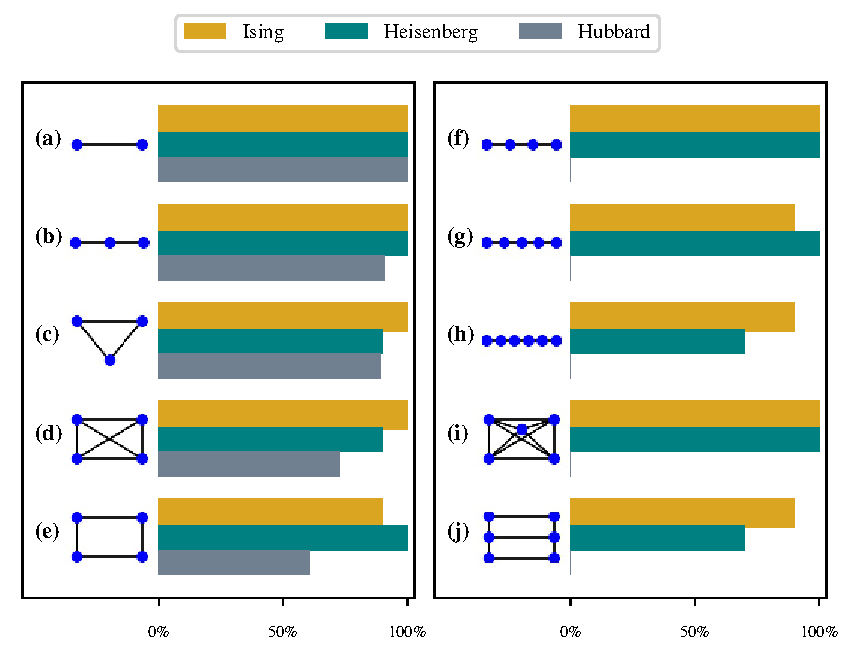
\includegraphics{theoretical_study/lattices/lattice_successes_two_column.pdf}
    \end{center}
    \caption{
        Rates of success for \gls{qmla} under various conditions. 
        Each lattice is set as the true model $\ho$ for ten independent instances. 
        In each instance, the \gls{es} considers the available lattices 
            (\textbf{a-j} for Ising and Heisenberg cases and \textbf{a-e} for the Hubbard case), 
            and selects a champion model $\hp$ as that most consistent with data generated by $\ho$. 
        The figure displays the rate at which each lattice is correctly identified as $\ho$
            under standard Ising, Heisenberg and Hubbard formalisms. 
        \figtableref
    }
    \label{fig:lattice_success_rates}
\end{figure}    

